%--------------------
% PARTIE 1 : Contexte
%--------------------

\section{Contexte du stage}
\label{chp:part1:context}

\subsection{Présentation de l'entreprise}
\label{chp:part1:presentation_company}

STMicroelectronics (ou ST) est une société internationale d’origine
franco-italienne.  STMicroelectronics est l’un des leaders mondiaux de la
conception et fabrication de semi- conducteurs.  La société est issue de la
fusion en 1987 de deux entreprises possédées par un gouvernement
(respectivement français et italien) : Thomson Semiconducteurs et SGS
(Societa Generale Semiconduttori). Le secteur d’activité de STMicroelectronics
à cette époque a évolué de l’électronique à destination de l’énergie nucléaire
et de l’électroménager vers l’informatique et les télécommunications.  La
première entrée en bourse de ST a été en 1994 avec la bourse de Paris et de
New York.  En 1998, ST s’est positionnée comme le 14 ème fournisseur mondial de
semi-conducteurs, en 2005 comme le plus grand fournisseur européen de semi-conducteurs
, devant Infineon et NXP (ex Philips Semiconductors), et comme le 5ème
fournisseur mondial de semi-conducteurs derrière Intel, Samsung, Texas
Instruments et Toshiba. On retrouve ainsi une majorité d'entreprises
concurrentes situées aux États-Unis (Intel, Qualcomm) ainsi qu'en Asie du
Sud-Est (Samsung, Toshiba). \\

STMicroelectronics fournit un effort conséquent pour l’innovation, avec 7 400
de ses 46 000 employés travaillant en recherche et développement.
L’entreprise a déposé environ 18 000 brevets parmi 9 600 familles de brevets
différentes.  En 2018, environ 15\% des revenus ont été dédiés à la recherche
et au développement, avec 500 nouveaux brevets déposés.  Ce fort
investissement dans la recherche a permis de positionner STMicroelectronics
comme acteur clé dans les technologies nouvelles générations, avec des
microcontrôleurs très basse consommation, des composants de gestion d’énergie,
de protection, des capteurs et actionneurs MEMS, ainsi que des puces de
connectivité et de contrôle moteur. \\

Aujourd’hui, les thématiques de STMicroelectronics sont la conduite augmentée
(Smart Driving) et l’internet des objets (Internet of Things). Le secteur
internet des objets se décompose en trois sous-thématiques : les objets
connectés (Smart Things), la domotique et la ville intelligente (Smart Home
and City) et l’industrie augmentée (Smart Industry). \\

Les familles de produits issues de ces thématiques sont les circuits intégrés
numériques à applicatif spécifique (ASIC numériques), les EEPROMs et
microcontrôleurs polyvalents, les MEMS , les capteurs d’imagerie spécialisée,
les circuits intégrés analogues, industriels et de gestion d’énergie, les
circuits intégrés dédiés à l’automobile et les transistors de puissance. \\

En interne, cela se traduit en trois groupes de développement : Automobile et
circuits discrets (ADG, Automotive and Discrete IC Group), MEMS et circuits
analogiques (AMG, AnalogIC and MEMS Group) et microcontrôleurs et circuits
digitaux (MDG, Micro-controllers and Digital IC Group). \\

\begin{figure}[H]
    \begin{center}
        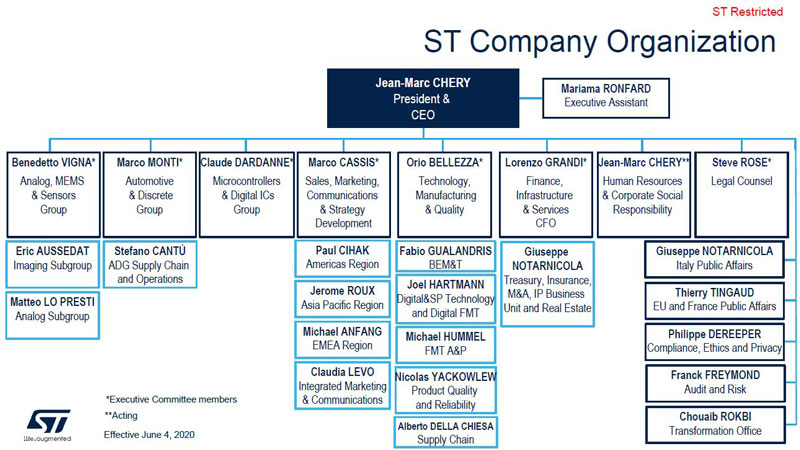
\includegraphics[width=\textwidth]{\pathPartOne/organigramme}
        \caption{Organigramme du comité exécutif ST}
        \label{fig:organigramme}
    \end{center}
\end{figure}

L’organisation hiérarchique de STMicroelectronics est très complexe du fait de
sa taille et son ampleur considérable. Dû à son affiliation franco-italienne,
l’exercice de toutes les fonctions requises pour son développement et la
gouvernance se font d’abord par un Comité de Direction. Celui-ci est composé
de huit personnes, correspondant à chaque division citée précédemment en plus
des structures financières et législatives et supervisé par M.  Jean-Marc
Chery, industriel ST diplômé de l'ENSAM Paris-Tech. Il est par ailleurs à
noter que le maintien législatif du groupe possède deux responsables des
affaires publiques pour chaque gouvernement, respectivement français et
italien. \\

À un niveau plus local, au Mans, la société Philips implémente un centre de
recherche et développement sur la technologie GSM, et fait de ce site le siège
de l’équipe « Philips Consumer Communication » en 1994. En 2001, suite à
l’arrêt pour Philips de la production de téléphones portables, une partie de
l’équipe de recherche rejoint « Philips Semiconductors » et en 2006, Philips
vend « Philips Semiconductors » qui deviendra NXP. \\

La branche «Mobile and Personal » de NXP a été cédée en 2008 au profit de la
création d’une coentreprise, ST-NXP Wireless, détenue à 80\% par
STMicroelectronics et à 20\% par NXP.  En 2009, STMicroelectronics fait
l’acquisition totale de ST-NXP Wireless pour fonder aux côtés de l’équipe «
Mobile Platform » d’Ericsson la coentreprise ST-Ericsson (détenue à parts
égales). ST- Ericsson a beaucoup contribué au développement de modems intégrés
(les NovaThor). En 2013, suite à la dissolution de ST-Ericsson, le site du
Mans rejoint STMicroelectronics. \\

\begin{figure}[H]
	\begin{center}
		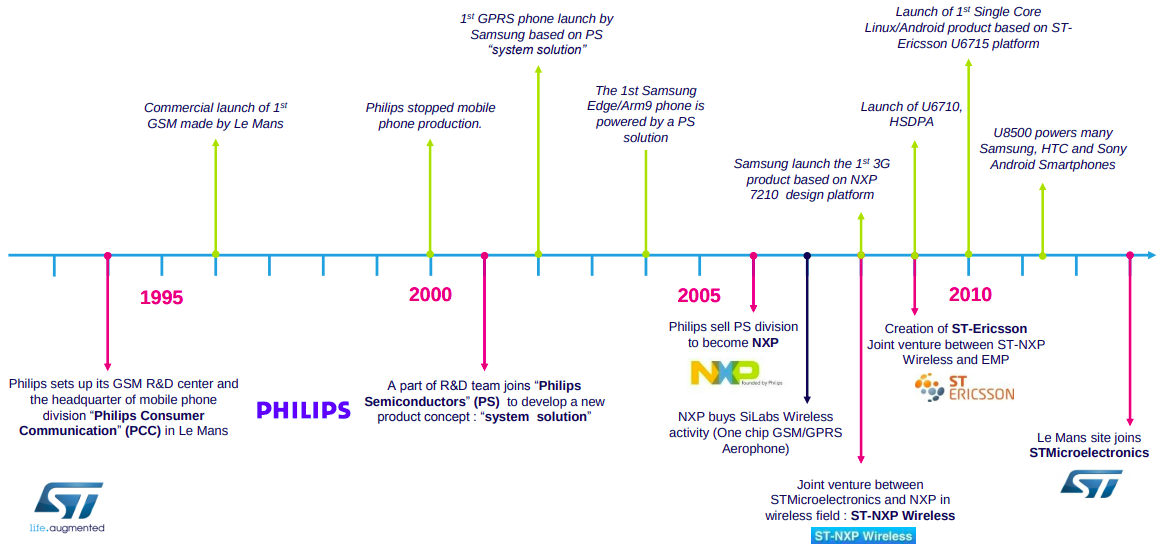
\includegraphics[width=\textwidth]{\pathPartOne/st_timeline}
                \caption{Chronogramme du site ST Le Mans}
	    \label{fig:st_timeline}
	\end{center}
\end{figure}

Aujourd'hui, le site du Mans est composé d’environ 225 employés, dont 95\%
d’ingénieurs.  Sur ces 225 employés, 118 employés (soit 52,4\%) font partie du
regroupement « Micro-controllers and Digital IC Group », 96 employés (soit
42,7\%) font partie du regroupement « Automotive and Discrete IC Group », et
enfin 11 employés (soit 4.9\%) font partie de l’équipe support. Le site du
Mans ne possède pas de division AMG. L’équipe liée au développement des
microprocesseurs (ou équipe MPU) est composée d’environ 60 employés de MDG,
dont 30 font partie de l’équipe de développement logiciel MPU dirigé par M.
Philippe Peurichard. \\

ST Le Mans est dirigé par M. Jérôme Bourgeais. Au sein de la division MPU,
parmi laquelle j'étais intégré, on retrouve des sous-groupes, nommés domaines.
Il y a par exemple le domaine Visual, traitant des pilotes autour des écrans,
touch screens et caméras, le domaine Core s'occupant de l'aspect des pilotes
Ethernet et communications ou encore Power pour la gestion de l'alimentation
du MPU. On remarquera que l'équipe "Kernel" n'existe pas pour la simple raison
que tous les domaines ont un mainteneur qui intègre le noyau Linux. \\

\subsection{Présentation des acteurs}
\label{chp:part1:presentation_actors}

Le mode de fonctionnement de cette expérience professionnelle s'inscrit dans
le cycle de développement du monde Open Source.  Effectivement, il est
désormais impossible pour une entreprise de ne pas bénéficier des logiciels
libres. En effet, chaque fonctionnalité vouée à être publiée au sein d'un
projet Open Source est passée en revue par des experts dans leur milieu. On a
donc une qualité et une sûreté de fonctionnement provenant du code intégré au
projet. Ensuite, comme l'Open Source possède l'avantage d'une gratuité de
diffusion, une entreprise lambda peut quasiment s'affranchir du coût de
maintenance puisqu'au delà de la maintenance locale à l'entreprise, des
développeurs extérieurs à l'organisation peuvent s'en charger. Enfin la
participation de nombreuses entreprises diversifie les besoins qu'un seul et
même projet doit prodiguer, et augmente par conséquent la modularité de son
code source. On retrouve ainsi une communauté d'entreprises et de particuliers
grandissante dans la participation à des projets Open Source. Pour prendre
l'exemple du noyau Linux, on retrouve de plus en plus d'applications dans le
domaine des systèmes embarqués, domaine dans lequel le noyau Linux n'était pas
destiné il y a moins d'une dizaine d'années. On peut le remarquer avec le
nombre croissant de contributeurs parmi le noyau Linux. \\

\begin{figure}[H]
	\begin{center}
		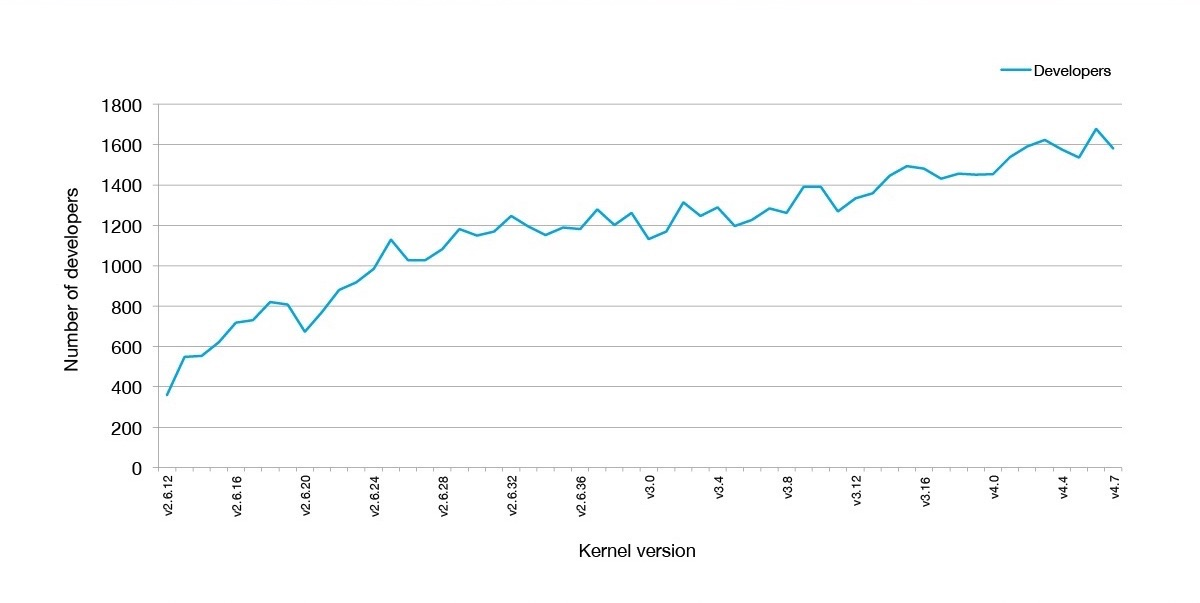
\includegraphics[width=\textwidth]{\pathPartOne/Linux-kernel-contributors-graph}
		\caption{Nombre de contributeurs au projet Linux suivant les versions}
	    \label{fig:contributors_graph}
	\end{center}
\end{figure}

Travailler au sein d'un large projet Open Source implique également un partage
à une communauté. Cette communauté se distingue en quatre catégories d'acteurs :

\begin{itemize}[label=\textbullet]
    \item Les mainteneurs
    \item Les committers ou développeurs
    \item Les contributeurs
    \item Les utilisateurs
\end{itemize}

Les utilisateurs sont les consommateurs finaux utilisant le produit. Ce sont
les acteurs les plus importants dans la mesure où ce sont eux qui répondent
directement au besoin du projet. Ici, ce sont donc les utilisateurs de la
distribution Linux publiée par ST. Les contributeurs sont des utilisateurs un
peu plus impliqués dans la conception du projet. Comme leur nom l'indique, ils
contribuent à des tâches annexes telles que la documentation, traduction,
faire des rapports de bogues sur les plateformes dédiées ou encore participent
à des campagnes de tests. Les committers sont des personnes ayant acquis une
notoriété suffisante au sein de la communauté pour s'être vu octoyer les
droits de modifier le code source. Ce sont pour ainsi dire des développeurs,
participant activement au progrès du projet. Enfin viennent les mainteneurs
qui sont des acteurs pouvant organiser des portions du code source et
approuvant l'intégration des fonctionnalités créées par les committers. Les
mainteneurs peuvent se décliner en sous-groupes de telle manière que plusieurs
mainteneurs "délégués" se chargent de l'intégration de parties spécifiques du
projet. \\

Au travers des différentes interactions entre ST et le monde extérieur, on
retrouve ainsi Linaro qui est un consortium d'entreprises dont l'objectif est
de développer et médiatiser le logiciel libre sur les architectures de type
ARM.  Linaro fait partie des 10 plus grands contributeurs au projet du noyau
Linux, et compte environ 250 ingénieurs répartis dans le monde entier. Ce
consortium inclus des entreprises telles que ARM, ST, Samsung, NXP ou encore
Google.  Parmi les acteurs décisifs de la mission qui m'a été confiée, on
retrouve Mathieu Poirier, ingénieur chez Linaro et mainteneur du sous-système
Coresight. C'est également la raison pour laquelle des échanges ont été
effectués avec lui. \\

% ARM, ST, Linaro, la communauté, Mathieu Poirier
Pour résumer, on a 4 grands acteurs de la communauté Linux pour cette mission
: ARM délivrant les blocs matériels (processeurs, sous-systèmes Coresight...),
ST chez qui le microprocesseur est conçu, et enfin Linaro. \\

\subsection{Déroulement du cycle d'un projet Open Source}

%Le cycle de développement d'un projet Open Source 
Tous ces acteurs assurent donc une pérennité du projet sur le long terme selon
un cycle de développement orienté de l'utilisateur vers le mainteneur.
L'émergeance de cette notion de remonter les informations se traduit au niveau
des committers et mainteneurs qui "upstreament" leurs nouveautés dans l'arbre
du projet principal. En pratique, les développeurs vont implémenter une
fonctionnalité répondant au besoin utilisateur et une fois validée, l'envoyer
sous forme de patch aux mainteneurs responsable de la branche. Le mainteneur
va tout d'abord inspecter si ce patch est conforme aux normes instaurées par
le projet, puis l'approuver. Dans le cas contraire, un feedback va être fait
au committer pour qu'il revoit la conception de sa fonctionnalité, d'où le
lien étroit entre développeurs et mainteneurs. Finalement, le mainteneur va
publier le patch pour une future version du projet. Cela est illustré par la
figure \ref{fig:linux_kernel_dev_process} ci-contre. \\

\begin{figure}[H]
	\begin{center}
		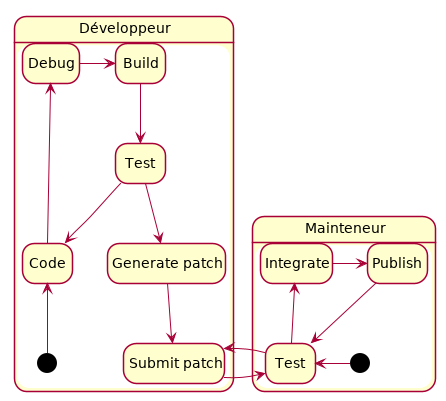
\includegraphics[scale=0.6]{\pathPartOne/linux_kernel_dev_process}
		\caption{Diagramme du processus de développement du noyau Linux}
	    \label{fig:linux_kernel_dev_process}
	\end{center}
\end{figure}

% Section économique (+ tableau?)
% Valeurs + actionnaires
% Concurrence: https://fr.wikipedia.org/wiki/Liste_des_principaux_fabricants_de_semi-conducteurs_au_fil_des_ans#Classement_2015
% Actors: https://www.linuxfoundation.org/resources/open-source-guides/participating-open-source-communities/
% Licences and juridics: https://open-source.developpez.com/tutoriels/guide-open-source/#LVII-A-2-a-i
% Linux Kernel dev process: https://www.kernel.org/doc/html/v4.15/process/2.Process.html
% https://thewalkingdeadfrance.org/global-microprocessor-market-covid-updates-3/
% https://en.wikipedia.org/wiki/Arm_Holdings
